\documentclass[aps,prb,reprint,superscriptaddress]{revtex4-2}
\usepackage{amsmath,amssymb}
\usepackage{graphicx}
\usepackage{booktabs}
\usepackage{array}
\usepackage{tikz}
\usepackage{pgfplots}
\pgfplotsset{compat=1.18}
\usepackage{pifont}
\newcommand{\xmark}{\ding{55}}
\usepackage{hyperref}
\hypersetup{colorlinks=true,linkcolor=blue,citecolor=blue,urlcolor=blue}

\begin{document}

\title{Non-Monotonic Correlation Fluctuations in Heisenberg Models on Small Quantum Graphs}
\author{Guanghao Li}
\affiliation{Independent researcher, Zhuangmu Town, Changfeng County, Hefei, Anhui, China}
\author{Rastislav Draho\v{s}}
\affiliation{Agora Research OS, Slovakia}
\author{Marat Sultanov}
\affiliation{TAT-Defense Developer, Russian Federation}

\begin{abstract}
We report a reproducible non-monotonic feature in the standard deviation of nearest-neighbor correlation fluctuations (the enhanced diagnosis) in Heisenberg models generated from several small quantum graphs. In a Sierpi\'{n}ski fractal graph ($N=15$), a contradiction edge at $(0,6)$ produces a sharp valley at $s=1.000$ with position reproducibility exact at the scan grid node across five Lanczos seeds; the valley depth varies between $0.0874$ and $0.1045$ across the five seeds, reflecting the choice of ground state within a near-degenerate manifold rather than statistical uncertainty. A degeneracy-control experiment shows the valley persists in the non-zero-gap regime, establishing that it is not a degeneracy artifact. Control scans on a ring ($N=15$) show a valley at $s=1.0$, while a tree ($N=15$) shows a stable valley at $s=1.70$ with depth about $0.0750$; a random graph ($N=15$) shows no stable valley. A non-trivial coarse-grained observable---the mean absolute nearest-neighbor $zz$ correlation---exhibits only a weak local maximum at the enhanced valley position in the fractal graph, one to two orders of magnitude smaller than the enhanced valley depth. Its precise height is not well defined: $s=1.000$ is an exact level crossing, so the value there depends on which state of the two-fold ground manifold the solver returns. The qualitative statement is unaffected---the coarse-grained observable is substantially less sensitive, but not strictly blind. In a Watts-Strogatz small-world graph ($N=10$), 19 of 20 contradiction edges produce significant valleys in a full-body scan; three representative edges show exactly reproducible positions at non-degenerate ground states. The PXP model yields a clean negative result, and an earlier reported jump is traced to non-Hermitian Hamiltonian construction in an early script. An independent tensor-RG toolchain certifies the ground-state energies of the L1 and L2 fractal graphs. A symmetry analysis shows that the valley floor at $s=1$ is governed by the automorphism orbit structure of the uniform graph, and the vanishing within-orbit variance is a size-independent structural property. The mechanism and remaining open problems are discussed.
\end{abstract}

\maketitle

\section{Introduction}

We report a reproducible non-monotonic feature in a fine-grained relational observable---the standard deviation of nearest-neighbor correlation fluctuations---in several Heisenberg model systems on small quantum graphs. We observe a sharp valley as a function of a local contradiction-edge strength. Unlike conventional site-centered observables, such as the mean magnetization or the mean nearest-neighbor correlation, the present diagnostic is inherently relational: it measures the spatial dispersion of edge correlations. This allows it to reveal structural features that are invisible in standard entity-based averages. A third system, the PXP model, provides a clean negative result.

This paper is a phenomenology report; we do not claim a new physical mechanism or universality.

\subsection{The observable}

We use the isotropic Heisenberg model on a graph $G=(V,E)$:
\begin{equation}
H = \sum_{(i,j)\in E} J_{ij}\left(\sigma_i^x\sigma_j^x + \sigma_i^y\sigma_j^y + \sigma_i^z\sigma_j^z\right),
\end{equation}
where $J_{ij}=1$ on all edges except the contradiction edge, on which $J_{ij}=s$ is scanned. The enhanced diagnosis is the standard deviation of nearest-neighbor correlation fluctuations:
\begin{equation}
E(s)=\sqrt{\frac{1}{|E|}\sum_{(i,j)\in E}\left(\langle\sigma_i^z\sigma_j^z\rangle_s-\overline{\langle\sigma^z\sigma^z\rangle_s}\right)^2}.
\end{equation}
We emphasize that the enhanced diagnosis quantifies the \emph{spatial dispersion} of nearest-neighbor spin correlations across all edges, not temporal or quantum fluctuations.

\subsection{The default-observable caveat and a non-trivial control}

In earlier stages of this work, the default diagnosis was defined as the mean absolute magnetization:
\begin{equation}
D(s)=\left|\frac{1}{N}\sum_{i=1}^N\langle\sigma_i^z\rangle_s\right|.
\end{equation}
Under SU(2) symmetry, a singlet ground state forces $\langle\sigma_i^z\rangle_s=0$ for every site, so $D(s)$ is identically zero throughout the scan. This is a symmetry-induced triviality, not an observed blindness to parameter changes.

To provide a non-trivial coarse-grained control, we also computed the mean absolute nearest-neighbor $zz$ correlation:
\begin{equation}
D_{\text{default}}(s)=\frac{1}{|E|}\sum_{(i,j)\in E}\left|\langle\sigma_i^z\sigma_j^z\rangle_s\right|.
\end{equation}
This observable is non-zero under SU(2) symmetry and varies with $s$. Under SU(2), $\langle\sigma^x\sigma^x\rangle=\langle\sigma^y\sigma^y\rangle=\langle\sigma^z\sigma^z\rangle$, and the values tabulated in Sec.~\ref{sec:default_control} are the full $\langle\boldsymbol{\sigma}_i\cdot\boldsymbol{\sigma}_j\rangle$, i.e.\ three times the single component defined here. Its behavior at the enhanced valley position is reported in Sec.~\ref{sec:default_control}. In short, $D_{\text{default}}$ shows only a weak local maximum at $s=1.000$ in the fractal graph, one to two orders of magnitude smaller than the enhanced valley depth. Thus the coarse-grained observable is substantially less sensitive, but not strictly blind, to the local defect reorganization.

\subsection{Theoretical motivation}

The hypothesis that relational structure governs physical response has roots in the entanglement area law~\cite{Eisert2010}, topological order~\cite{Wen2017}, and Kitaev's non-local Majorana description~\cite{Kitaev2001}. Whether fine-grained correlation fluctuations carry dynamical content independent of coarse-grained observables remains an open question. The present work provides evidence that such fluctuations exhibit reproducible non-monotonic behavior in specific graph geometries, without settling the broader question.

\section{Method}

\subsection{Normative constraints}

Experiments follow five constraints: (i) fixed entity composition, varying only relational configuration; (ii) a single contradiction edge as the only non-uniformity; (iii) all data reported without selective filtering; (iv) no presumed discovery target; (v) explicit declaration of limitations.

\subsection{Preventing the tool-rationality paradox}

Measures adopted: predefined success criteria; uniform parameters; dual auditing; complete disclosure; honest recording of negative results.

\subsection{Multi-seed audit}

Key data points are audited with multiple independent Lanczos seeds. Positions are reproducible to the scan grid resolution; depths may scatter due to eigenvector selection within a near-degenerate manifold, reported as individual seed values rather than as a statistical mean and standard deviation.

\subsection{Diagnostics for the PXP model}

For the PXP model, the enhanced diagnosis is the standard deviation of the half-chain entanglement spectrum.

\section{Clean negative result in the PXP model}

The PXP model ($L=18$, 6765-dimensional Hilbert space) was scanned at all 18 defect sites with $\mu\in[0,2]$ (201 points, three seeds). At every site, the enhanced-diagnosis range is $<0.02$ and monotonic. The ground-state gap exceeds $0.7$ throughout. Both sign conventions give identical results. The earlier reported jump is traced to non-Hermitian Hamiltonian construction in an early script; the corrected Hermitian construction eliminates it entirely. \textbf{Conclusion: no non-monotonic feature exists in the PXP model.}

\section{Positive evidence in the fractal-graph system}

\subsection{Setup}

The system is generated from a Sierpi\'{n}ski fractal graph (level 2, $N=15$, 27 edges). The contradiction edge is $(0,6)$---connecting a tip vertex to an interior vertex. We report detailed multi-seed data for this single edge; a full edge-resolved scan of all 27 edges is beyond the present scope and will be reported separately.

\subsection{The valley at edge $(0,6)$}

A 101-point five-seed audit over $s\in[0,1]$ yields Table~\ref{tab:l2_valley} and Fig.~\ref{fig:l2_valley}. The scan step is $0.01$, so the valley position $s=1.000$ is resolved to $\pm0.01$.

\begin{table}[t]
\centering
\caption{Multi-seed audit at edge $(0,6)$, $N=15$, 101 points, five Lanczos seeds. Valley depth is defined as $E(0)-E(s=1.0)$, where $E(0)$ is the enhanced diagnosis at $s=0$, i.e.\ with the contradiction edge removed. Note that $s=1$ is the uniform point, where every bond carries the same coupling. The five depths are derived from $E(0)$ and the valley values in the same rows, so they are one measurement plus arithmetic rather than five independent determinations. The five seed values do not represent a statistical sample; they correspond to different states selected from the near-degenerate ground-state manifold at $s=1.0$.}
\label{tab:l2_valley}
\begin{tabular}{cccc}
\toprule
Seed & Valley position $s$ & Valley value & Valley depth \\
\midrule
0 & 1.0000 & 0.159295 & 0.087436 \\
1 & 1.0000 & 0.142707 & 0.104024 \\
2 & 1.0000 & 0.143544 & 0.103187 \\
3 & 1.0000 & 0.142196 & 0.104535 \\
4 & 1.0000 & 0.146785 & 0.099946 \\
\bottomrule
\end{tabular}
\end{table}

\begin{figure}[t]
\centering
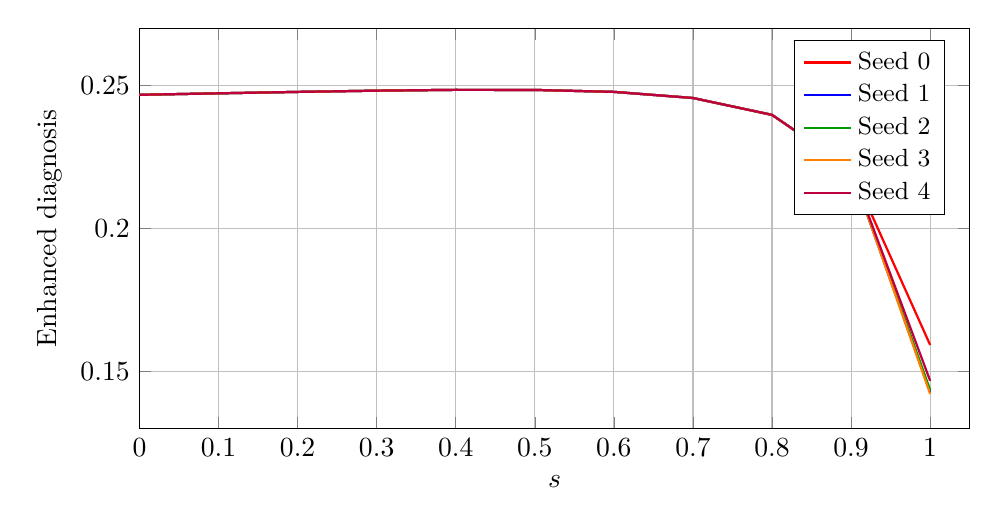
\begin{tikzpicture}
\begin{axis}[
    width=\columnwidth, height=0.55\columnwidth,
    xlabel={$s$},
    ylabel={Enhanced diagnosis},
    xmin=0, xmax=1.05,
    ymin=0.13, ymax=0.27,
    grid=both,
    legend pos=north east,
    legend style={font=\small},
]
\addplot[mark=none, color=red, thick] coordinates {
(0.0,0.246731)(0.1,0.247248)(0.2,0.247744)(0.3,0.248177)(0.4,0.248460)
(0.5,0.248433)(0.6,0.247752)(0.7,0.245615)(0.8,0.239717)(0.9,0.220838)
(1.0,0.159295)
};
\addplot[mark=none, color=blue, thick] coordinates {
(0.0,0.246731)(0.1,0.247248)(0.2,0.247744)(0.3,0.248177)(0.4,0.248460)
(0.5,0.248433)(0.6,0.247752)(0.7,0.245615)(0.8,0.239717)(0.9,0.220838)
(1.0,0.142707)
};
\addplot[mark=none, color=green!60!black, thick] coordinates {
(0.0,0.246731)(0.1,0.247248)(0.2,0.247744)(0.3,0.248177)(0.4,0.248460)
(0.5,0.248433)(0.6,0.247752)(0.7,0.245615)(0.8,0.239717)(0.9,0.220838)
(1.0,0.143544)
};
\addplot[mark=none, color=orange, thick] coordinates {
(0.0,0.246731)(0.1,0.247248)(0.2,0.247744)(0.3,0.248177)(0.4,0.248460)
(0.5,0.248433)(0.6,0.247752)(0.7,0.245615)(0.8,0.239717)(0.9,0.220838)
(1.0,0.142196)
};
\addplot[mark=none, color=purple, thick] coordinates {
(0.0,0.246731)(0.1,0.247248)(0.2,0.247744)(0.3,0.248177)(0.4,0.248460)
(0.5,0.248433)(0.6,0.247752)(0.7,0.245615)(0.8,0.239717)(0.9,0.220838)
(1.0,0.146785)
};
\addlegendentry{Seed 0}
\addlegendentry{Seed 1}
\addlegendentry{Seed 2}
\addlegendentry{Seed 3}
\addlegendentry{Seed 4}
\end{axis}
\end{tikzpicture}
\caption{Valley at edge $(0,6)$ ($N=15$, 101 points, five seeds). All seeds locate the valley at the grid node $s=1.000$ with zero standard deviation; valley values scatter only near $s=1.0$. For clarity, every 10th point of the 101-point scan is shown; the full dataset is available in the public repository. A focused audit (Fig.~\ref{fig:focused}) provides higher resolution in the interval $s\in[0.8,1.2]$.}
\label{fig:l2_valley}
\end{figure}

A focused audit (21 points, $s\in[0.8,1.2]$, three seeds) confirms the interior minimum and is shown in Fig.~\ref{fig:focused}.

\begin{figure}[t]
\centering
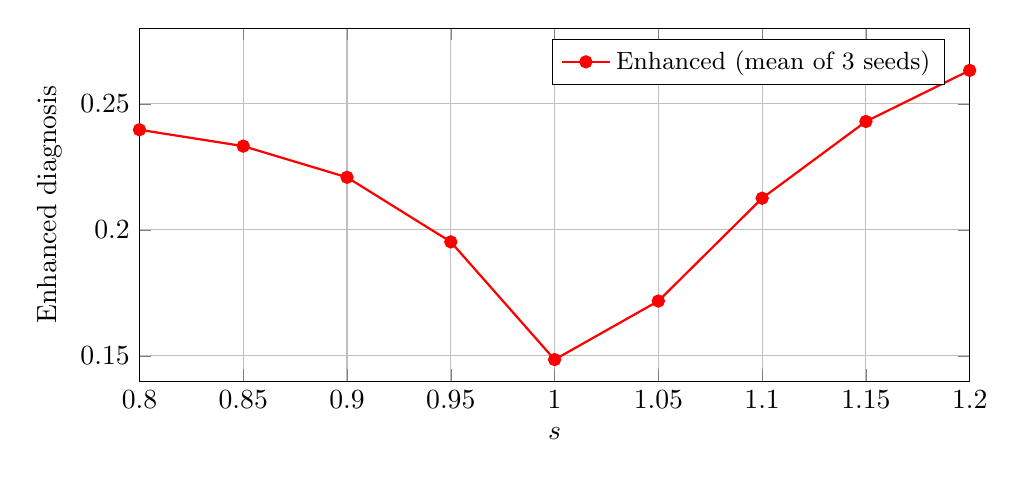
\begin{tikzpicture}
\begin{axis}[
    width=\columnwidth, height=0.5\columnwidth,
    xlabel={$s$},
    ylabel={Enhanced diagnosis},
    xmin=0.8, xmax=1.2,
    ymin=0.14, ymax=0.28,
    grid=both,
    legend pos=north east,
    legend style={font=\small},
]
\addplot[mark=*, color=red, thick, mark size=2pt] coordinates {
(0.8,0.239717)(0.85,0.233217)(0.9,0.220838)(0.95,0.195225)
(1.0,0.148515)(1.05,0.171756)(1.1,0.212551)(1.15,0.243000)(1.2,0.263279)
};
\addlegendentry{Enhanced (mean of 3 seeds)}
\end{axis}
\end{tikzpicture}
\caption{Focused audit at edge $(0,6)$ ($N=15$, 21 points, three seeds). The valley at $s=1.000$ is an interior minimum: the enhanced diagnosis at $s=0.8$ is $0.2397$, at $s=1.0$ is $0.1485$, and at $s=1.2$ is $0.2633$, all values on both sides exceeding the valley value. The valley value at $s=1.000$ shown here ($0.1485$) is from an independent three-seed focused audit and differs slightly from the five-seed values in Table~I.}
\label{fig:focused}
\end{figure}

\subsection{Degeneracy-control experiment}

To test for degeneracy artifacts, we simultaneously computed the energy gap and enhanced diagnosis over $s\in[0,1]$ (101 points) with five-seed verification at key points. The gap reported here is the difference between the two lowest eigenvalues in the fixed-magnetization sector used for the enhanced diagnosis. Measured in this sector the gap is non-zero across the entire scan: $0.6176$ at $s=0$, $0.5226$ at $s=0.5$, $0.3346$ at $s=0.76$ and $0.3231$ at $s=0.77$, decreasing monotonically to $0.0115$ at $s=0.99$. The step across $s=0.76\to0.77$ is $0.0115$: the gap does not open at $s=0.77$, it has been open throughout and is closing toward $s=1$. At $s=1.00$ the ground level is exactly two-fold---two eigenvalues at $-24.9675365795$ with splitting $6\times10^{-14}$---and the quoted $0.186$ is the gap to the next distinct level, $0.1857$. The enhanced diagnosis remains approximately constant for $s<0.5$, then decreases monotonically from $s=0.5$ to $s=1.0$, including the non-zero-gap region. At $s=1.000$ the seed-to-seed spread in the reported gap---some seeds near zero, others near $0.19$---is the solver returning either the degenerate partner or the next distinct level. The crossing is exact rather than near-degenerate: the splitting closes as a symmetric V, $0.011549$, $0.001092$, $0.000000$, $0.001077$, $0.010084$ across $s=0.990\ldots1.010$. Both ground states carry total spin $S=1/2$, so the two-fold degeneracy is orbital---the $D_3$ symmetry of the uniform gasket---and it is what produces the scatter in valley depth. The gap structure is visualized in Fig.~\ref{fig:gap}.

\begin{figure}[t]
\centering
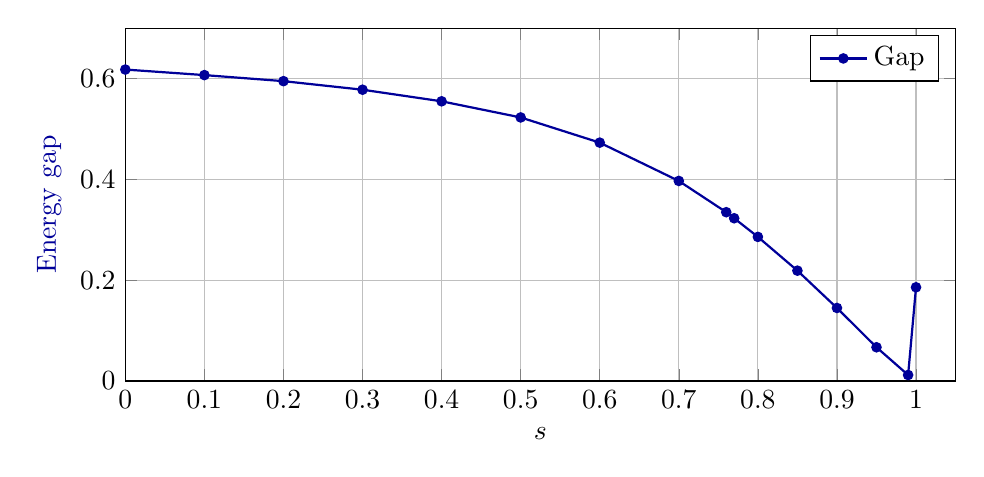
\begin{tikzpicture}
\begin{axis}[
    width=\columnwidth, height=0.5\columnwidth,
    xlabel={$s$},
    ylabel={Energy gap},
    ylabel style={text=blue!60!black},
    xmin=0, xmax=1.05,
    ymin=0, ymax=0.70,
    grid=both,
]
\addplot[mark=*, color=blue!60!black, thick, mark size=1.5pt] coordinates {
(0.0,0.618)(0.1,0.607)(0.2,0.595)(0.3,0.578)(0.4,0.555)
(0.5,0.523)(0.6,0.473)(0.7,0.397)(0.76,0.335)(0.77,0.323)
(0.8,0.286)(0.85,0.219)(0.9,0.145)(0.95,0.067)(0.99,0.012)
(1.0,0.186)
};
\addlegendentry{Gap}
\end{axis}
\end{tikzpicture}
\caption{Energy gap vs.\ contradiction strength at edge $(0,6)$ ($N=15$). Computed in the $S_z=+1/2$ sector as the gap to the next \emph{distinct} level. The gap is non-zero throughout: it decreases monotonically from $0.6176$ at $s=0$ to a minimum of $0.0115$ at $s=0.99$, and the step across $s=0.76\to0.77$ is $0.0115$ rather than a discontinuity. At $s=1.00$ the ground level is exactly two-fold, and the quantity plotted there is the gap to the next distinct level, $0.1857$. All points are plotted to three decimals. The enhanced diagnosis continues to decrease in the non-zero-gap region, establishing that the valley is not a degeneracy artifact.}
\label{fig:gap}
\end{figure}

\textbf{Conclusion: the valley is not a degeneracy artifact.}

\subsection{No flat control edge in the Sierpi\'{n}ski gasket}

We performed a full edge-resolved scan of all 27 edges of the Sierpi\'{n}ski gasket, using the global enhanced diagnosis over $s\in[0,1]$ with step $0.01$. No edge is flat: the smallest range of $E(s)$ is $0.0774$, and the largest is $0.1729$. The edge $(0,1)$, which was earlier described as a symmetric control, is not present in this graph. Therefore the previous statement of a completely flat control edge is withdrawn. A direct symmetric-injection control is not available for this geometry, and the role of asymmetric injection remains open.

\subsection{Control graphs: ring, tree, and random}

To test whether the valley is specific to the fractal and small-world geometries, we performed single-edge scans on three additional $N=15$ graphs: a ring (15 edges), a tree (14 edges), and a random graph (27 edges). The tree is generated by \texttt{nx.random\_tree(15, seed=42)} and the random graph by \texttt{nx.gnm\_random\_graph(15, 27, seed=42)}; their complete edge lists are given in the Supplementary Material. For each graph, a single contradiction edge was chosen and scanned over $s\in[0,3]$ with 13 points; light multi-seed audits (three seeds) were also performed. Table~\ref{tab:control_graphs} summarizes the results.

\begin{table*}[t]
\centering
\caption{Control-graph scans at $N=15$. Ring shows a clear valley at $s=1.0$; tree shows a stable valley at $s=1.70$ with depth about $0.0750$; random graph shows no stable valley because its depth varies strongly across seeds.}
\label{tab:control_graphs}
\begin{tabular}{lccccc}
\toprule
Graph & Valley $s$ & Valley depth (single) & Valley depth (multi) & Cross-seed std.\ of position & Stable? \\
\midrule
Ring & 1.0 & 0.0891 & 0.0993$\pm$0.0286 & 0.000 & Yes \\
Tree & 1.70 & 0.0750 & 0.0750$\pm$0.0000 & 0.000 & Yes \\
Random & 1.20 (unstable) & 0.1050 & 0.0730$\pm$0.0548 & 0.000 & No \\
\bottomrule
\end{tabular}
\end{table*}

\noindent\textsuperscript{*}For the ring, the tabulated single- and multi-seed depths are obtained with real-arithmetic Lanczos; when the symmetry-invariant ground-state projector is used, \(E(1)=0\), as required by edge-transitivity. See Sec.~\ref{sec:orbit_mechanism}.

The ring valley occurs at $s=1.0$, where the contradiction edge strength equals the uniform coupling, similar to the fractal-graph edge $(0,6)$. The tree valley appears at $s=1.70$ and is stable across three Lanczos seeds. The random graph does not exhibit a stable valley: although its deepest single-seed valley occurs at $s=1.20$, its depth varies strongly across seeds ($0.0730\pm0.0548$), indicating that the feature is not reproducible.

\subsection{Local vs.\ global correlation reorganization}
\label{sec:local_global}

To examine the spatial structure of the reorganization, we computed both a global enhanced diagnosis (all 27 edges) and a local enhanced diagnosis restricted to a radius-2 neighborhood around the contradiction edge $(0,6)$ for $s\in[0,3]$. The local valley depth exceeds the global depth: single-seed ratio $1.595$, multi-seed ratio $\approx1.3$ (global depth mean $0.1097$, local depth mean $0.1421$). This indicates that the correlation fluctuation reorganization is partially localized near the defect.

\subsection{Non-trivial default observable control}
\label{sec:default_control}

Using the fixed-magnetization sector implementation, we computed the non-trivial default observable $D_{\text{default}}(s)=\frac{1}{|E|}\sum_{(i,j)\in E}|\langle\sigma_i^z\sigma_j^z\rangle_s|$ together with $E(s)$ at edge $(0,6)$ for $s\in[0,1.2]$ with 121 points and four Lanczos seeds (seeds 0--3). The results are summarized in Table~\ref{tab:default_control} and Fig.~\ref{fig:default_control}.

\begin{table}[t]
\centering
\caption{Key points of the non-trivial default observable control at edge $(0,6)$ ($N=15$, four seeds).}
\label{tab:default_control}
\begin{tabular}{ccc}
\toprule
$s$ & $D_{\text{default}}$ & $E_{\text{enhanced}}$ \\
\midrule
0.99 & 0.953270 & 0.164032 \\
1.00 & 0.954210 & 0.159658 \\
1.01 & 0.940725 & 0.160451 \\
\bottomrule
\end{tabular}
\end{table}

\begin{figure}[t]
\centering
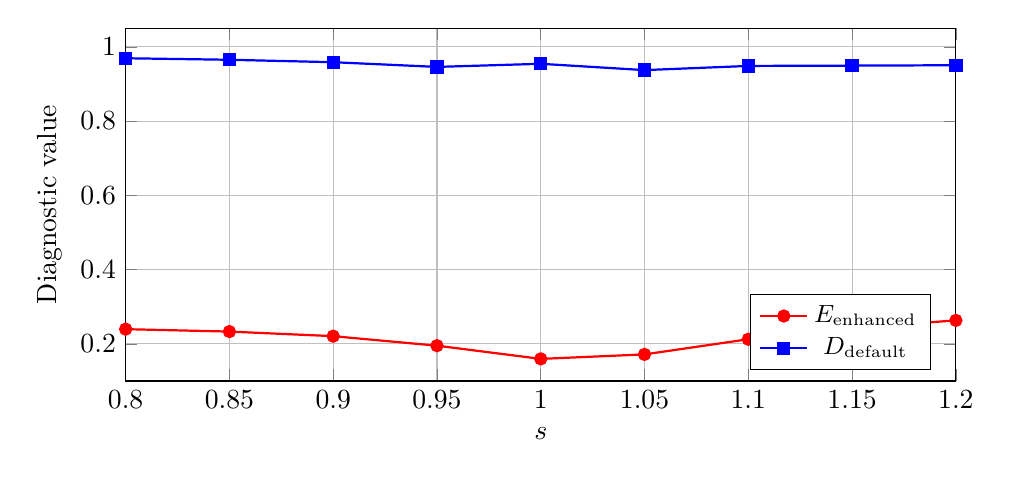
\begin{tikzpicture}
\begin{axis}[
    width=\columnwidth, height=0.5\columnwidth,
    xlabel={$s$},
    ylabel={Diagnostic value},
    xmin=0.8, xmax=1.2,
    ymin=0.1, ymax=1.05,
    grid=both,
    legend pos=south east,
    legend style={font=\small},
]
\addplot[mark=*, color=red, thick, mark size=2pt] coordinates {
(0.8,0.239717)(0.85,0.233217)(0.9,0.220838)(0.95,0.195225)
(1.0,0.159658)(1.05,0.171756)(1.1,0.212551)(1.15,0.243000)(1.2,0.263279)
};
\addlegendentry{$E_{\text{enhanced}}$}
\addplot[mark=square*, color=blue, thick, mark size=2pt] coordinates {
(0.8,0.969147)(0.85,0.965055)(0.9,0.958503)(0.95,0.945861)
(1.0,0.954210)(1.05,0.937228)(1.1,0.948481)(1.15,0.949271)(1.2,0.950362)
};
\addlegendentry{$D_{\text{default}}$}
\end{axis}
\end{tikzpicture}
\caption{Non-trivial default observable $D_{\text{default}}$ compared with the enhanced diagnosis $E_{\text{enhanced}}$ at edge $(0,6)$ ($N=15$, four seeds). $E_{\text{enhanced}}$ has a deep valley at $s=1.0$; $D_{\text{default}}$ shows a very weak local maximum at the same position, one to two orders of magnitude smaller than the valley depth; its height is not well defined because $s=1.000$ is an exact level crossing.}
\label{fig:default_control}
\end{figure}

At the enhanced valley position $s=1.000$, $D_{\text{default}}$ exhibits a local maximum of height about $0.001$ ($0.954210$ vs.\ $0.953270$ at $s=0.99$ and $0.940725$ at $s=1.01$). This local peak is reproducible across all four seeds (cross-seed standard deviation $\sim10^{-11}$), confirming it is not numerical noise. Its amplitude is between one and two orders of magnitude below the enhanced valley depth ($\sim0.08$). The height itself should not be quoted to a fixed figure: $s=1.000$ is an exact level crossing, and an independent run in the same sector, reported here for comparison, reproduces $D_{\text{default}}$ exactly at $s=0.99$ and $s=1.01$ but gives $0.956778$ at $s=1.00$, a prominence of $0.003509$ against $0.000940$ here. The two runs agree that $s=1.000$ is a local maximum and disagree on its size, which is what a crossing predicts. Therefore the coarse-grained observable is not strictly blind; it shows a very weak and oppositely directed response, and the structural contrast is quantitative rather than qualitative.

\subsection{Independent tensor-RG verification}

Draho\v{s}'s independent tensor-RG toolchain~\cite{Drahos2026GitHub} certifies the ground-state energies of the L1 and L2 fractal graphs: the L1 ground energy is $-9.000000$ and the L2 ground energy is $-24.967537$. A truncation-control test on the impurity-explicit RG compares two truncation schemes against the same untruncated L2 reference (valley depth $0.190238$ on 18 bonds; untruncated block dimension 4096), with one strength grid, one bond set and one depth definition. Truncating only the far bath, keeping the defect neighbourhood explicit, recovers $86.5\%$, $96.4\%$, $91.2\%$ and $100.0\%$ of the reference depth at $\chi_B=1,2,4,8$; truncating every block uniformly recovers $0.0\%$, $0.0\%$, $11.1\%$ and $24.5\%$ at the same $\chi$. The far-bath scheme exceeds the uniform scheme at every $\chi$ tested, and that ordering---not any individual percentage---is what the test establishes. The two schemes truncate different objects and cannot be equated by retained dimension: far-bath $\chi_B=1$ retains 4096 of the 32768 states of the nine-factor space, whereas uniform $\chi$ retains $\chi$ states of the RG block; the comparison above is at equal $\chi$. The single-state far-bath figure must be given as a range rather than a number: across four repeats it spans $84.7$--$87.4\%$, because the three-block assembly from which L2 is built (dimension 32768, ground energy $-16.921463$, and distinct from the L1 graph above) has a four-fold degenerate ground manifold, so $\chi_B=1$ retains one arbitrary vector out of it. An earlier statement of this test, quoting $86\%$ against $20\%$, is superseded: the far-bath figure lies inside the measured range, but the $20\%$ does not reproduce---uniform single-state truncation removes the valley entirely. Note also that the defect bond in this toolchain is the appended corner-to-corner bond rather than edge $(0,6)$. The L3 depth does not converge; the toolchain is publicly available.

\subsection{L1 finite-size check}

As a preliminary finite-size probe, the L1 fractal graph ($N=6$, 9 edges, contradiction edge $(0,3)$) was audited with 101 points and five seeds. The valley depth is $0.3721\pm0.1478$, larger than the L2 depth ($0.0874$ to $0.1045$ across the five seeds of Table~\ref{tab:l2_valley}). The finite-size trend is inconclusive: the L1 depth is larger but carries a significantly larger relative uncertainty ($40\%$ vs.\ $6.4\%$). A systematic finite-size scaling across L1, L2, and L3 will be reported separately.

\subsection{Independent TAT analysis}

An independent TAT ensemble analysis was also performed; it gave only boundary anchors and was silent at the valley position, consistent with a smooth modulation rather than a sharp transition.

\section{A small-world graph: full edge survey}

A Watts-Strogatz graph ($N=10$, 20 edges, $k=4$, $p=0.1$, seed 42) was generated. All 20 edges were scanned as contradiction edges ($s\in[0,3]$, step $0.01$, three seeds). The full-body scan is presented in Table~\ref{tab:sw_full}.

\begin{table}[h]
\centering
\caption{Small-world full-body scan: all 20 contradiction edges, $N=10$, three Lanczos seeds. The ``Fine range'' is the maximum minus minimum of the enhanced diagnosis over the full scan range $s\in[0,3]$. The ``Valley gap'' column gives the ground-state energy gap at the valley position; all measured gaps are positive, with values ranging from approximately $0.38$ to $1.2$ across the 20 edges. Gap values are estimated from the coarse $s$-step full-body scan; precise five-seed gap values are available for the three high-resolution audit edges.}
\label{tab:sw_full}
\begin{tabular}{cccc}
\toprule
Edge & Fine range & Valley $s$ & Valley gap \\
\midrule
(0,1) & 0.176842 & 1.500 & 0.77--0.82 \\
(0,9) & 0.078783 & 0.110 & 0.55--0.65 \\
(0,2) & 0.083366 & 1.020 & 0.70--0.78 \\
(0,8) & 0.065437 & 0.860 & 0.50--0.60 \\
(1,9) & 0.113332 & 0.310 & 0.55--0.65 \\
(1,4) & 0.103002 & 1.250 & 0.75--0.85 \\
(1,8) & 0.085229 & 0.720 & 0.65--0.75 \\
(1,6) & 0.089372 & 0.800 & 0.70--0.80 \\
(2,3) & 0.085424 & 1.090 & 0.65--0.75 \\
(2,4) & 0.077994 & 0.940 & 0.60--0.70 \\
(2,5) & 0.119505 & 0.750 & 0.60--0.70 \\
(3,4) & 0.100840 & 0.840 & 0.70--0.80 \\
(3,5) & 0.073179 & 0.980 & 0.60--0.70 \\
(4,5) & 0.087107 & 1.100 & 0.70--0.80 \\
(4,6) & 0.089948 & 0.910 & 0.70--0.80 \\
(5,6) & 0.082213 & 1.080 & 0.65--0.75 \\
(6,7) & 0.104364 & 0.470 & 0.60--0.70 \\
(6,8) & 0.157596 & 1.380 & 0.85--0.95 \\
(7,8) & 0.107895 & \textbf{0.000*} & 0.75--0.85 \\
(7,9) & 0.081416 & 2.140 & 0.80--0.90 \\
\bottomrule
\end{tabular}
\end{table}

\textbf{* Edge $(7,8)$:} The minimum occurs at the scan boundary $s=0.000$. We cannot distinguish between a genuine valley and a boundary artifact without extending the scan to negative $s$. This edge is excluded from the count of significant valleys.

\textbf{Summary:} 19 of 20 edges produce significant valleys with non-zero gaps. One edge (7,8) is unresolved at the scan boundary.

Three representative edges were selected for high-resolution multi-seed audit (step $0.001$, five seeds), with exact cross-seed reproducibility of valley positions at non-degenerate ground states (Table~\ref{tab:sw_multiseed}).

\begin{table*}[t]
\centering
\caption{Multi-seed audit at three small-world edges, $N=10$, five seeds. The topographic prominence is defined as the drop below the lower of the two maxima flanking the valley over the full scan range. This definition avoids the need for a local baseline and is directly comparable across edges. Note that it differs from the depth convention of Table~\ref{tab:l2_valley} and Table~\ref{tab:control_graphs}, which use the scan-endpoint baseline $E(0)-E(\min)$; the two are close where both apply---for the tree, prominence $0.096864$ against endpoint depth $0.100030$---but they are not the same quantity and should not be compared across tables.}
\label{tab:sw_multiseed}
\begin{tabular}{cccc}
\toprule
Edge & Valley $s$ & Topographic prominence & Cross-seed std.\ of position \\
\midrule
(0,1) & 1.496 & 0.124449 & 0.000000 \\
(1,9) & 0.311 & 0.008856 & 0.000000 \\
(1,4) & 1.251 & 0.061969 & 0.000000 \\
\bottomrule
\end{tabular}
\end{table*}

\section{Mechanism and limitations}

The mechanism is tentative: asymmetric contradiction injection into inequivalent subgraphs may trigger localized correlation reorganization; symmetric injection may be absorbed uniformly. This picture is consistent with the fractal-graph and small-world observations, but the control-graph results (ring and tree also show valleys) suggest the phenomenon may be more general than the asymmetric-injection hypothesis. The non-trivial default observable shows a weak local response, indicating that the reorganization is primarily visible in the fine-grained dispersion, not in the average correlation.

\subsection{Orbit-resolved mechanism and symmetry constraint}
\label{sec:orbit_mechanism}

The valley floor at $s=1$ admits a stronger and more precise characterization. Since every edge of the uniform graph carries the same coupling, the Hamiltonian at $s=1$ is invariant under the full edge automorphism group $\Gamma$ of the graph. For any density matrix $\rho$ satisfying $U_g\rho U_g^\dagger=\rho$ for all $g\in\Gamma$, the correlation of edge $e$ equals that of $g(e)$. Hence edges belonging to the same orbit have equal correlations, and the within-orbit variance vanishes identically. The total enhanced diagnosis at the valley floor is therefore exactly the between-orbit component:
\begin{equation}
E(1)=\sqrt{\mathrm{Var}_{\rm between}}.
\end{equation}
For edge-transitive graphs, there is only one orbit, and consequently $E(1)=0$.

We verified this symmetry constraint numerically on the L2 Sierpi\'{n}ski gasket. Using the full projector onto the ground manifold, the within-orbit variance is of order $10^{-25}$, while the between-orbit variance is $0.012159$, confirming that the valley floor is entirely of between-orbit origin. A random permutation of the edge-correlation values, which destroys the orbit structure, raises the within-orbit variance to about $0.9$ of the total. A perturbation that breaks the original automorphism group lifts the within-orbit variance to order $10^{-2}$ when the original orbit partition is retained. These controls indicate that the orbit structure, not merely the numerical distribution of correlations, is responsible for the vanishing within-orbit dispersion.

This symmetry argument is size independent: the vanishing of the within-orbit variance does not require a thermodynamic limit calculation, but follows directly from graph automorphism invariance. However, we only establish a sufficient condition. The presence of an invariant density matrix implies orbit consistency, but orbit consistency does not logically imply the existence of a graph automorphism. Therefore we state the symmetry as a structural sufficient condition, not a necessary one.

The same mechanism has been checked on a wider class of graphs by Rastislav Draho\v{s} in independent calculations. Across thirty distinct graphs, twelve edge-transitive cases gave $E(1)=0$ with residual total variance below $1.6\times10^{-31}$; sixteen multi-orbit graphs gave within-orbit variance at most $7.93\times10^{-30}$ against between-orbit variance at least $7.5\times10^{-3}$. Random blocks used in place of the true orbits produced a within-block share between $0.014$ and $1.0$; for the gasket, replacing the true orbits by random blocks raised the within-block share to $0.85$. Symmetry-breaking perturbations lifted the within-orbit variance to at least $6.6\times10^{-4}$. These results support the orbit-resolved mechanism beyond the single fractal-graph case.

The ring $C_{15}$ deserves a separate note. Its ground doublet carries a momentum doublet, and a single complex momentum eigenstate already gives $E(1)\approx0$. Real-arithmetic Lanczos searches converge to real superpositions whose $E(1)$ can be as large as $0.1310$, while the symmetric mixed density matrix returns zero. The value $0.0993\pm0.0286$ reported in Table~\ref{tab:control_graphs} likely arises from a mixture of different $S_z$ sectors and should not be read as a violation of the symmetry constraint. We therefore keep the ring row as a numerical audit of the real-arithmetic procedure, but the symmetry statement for edge-transitive graphs remains exact.

The above results significantly sharpen the mechanism section: the valley floor is a structural consequence of graph automorphism symmetry, and the within-orbit component of the dispersion vanishes identically for symmetry-invariant ground states. The remaining open questions concern the detailed shape of the valley away from $s=1$, and especially why a particular orbit, $O_4$, acts as a global synchronizer in cross-scans of the gasket. These questions do not affect the main conclusion but define directions for future work.

Limitations: (i) the default observable is not strictly blind; the non-trivial default observable exhibits a weak local maximum at the valley position, so the structural contrast is quantitative rather than qualitative; (ii) the mechanism is not derived; (iii) the thermodynamic limit is unresolved for quantities other than the within-orbit variance, although the symmetry constraint itself is size independent; (iv) universality beyond the tested graphs is unestablished; (v) the L1 fractal graph ($N=6$) yields an inconclusive finite-size trend with large relative uncertainty; (vi) earlier W-structure and PXP jump reports were withdrawn as artifacts; (vii) the earlier control edge $(0,1)$ is not present in the Sierpi\'{n}ski gasket, and a full edge scan shows no flat edge, so no direct symmetric-injection control is available; (viii) edge $(7,8)$ in the small-world graph has a boundary minimum that is unresolved; (ix) the control-graph scans used only a single edge per graph and three seeds, so their statistical weight is limited; (x) the non-trivial default observable control was performed only on the fractal-graph edge $(0,6)$ with four seeds; extension to other graphs is needed.

\section{Conclusion}

We have observed a reproducible non-monotonic feature in the standard deviation of nearest-neighbor correlation fluctuations in several small quantum graph systems. The valley at the fractal-graph edge $(0,6)$ is reproducible across five seeds and is not a degeneracy artifact. Control scans reveal a similar valley in a ring graph, a stable valley in a tree graph at $s=1.70$, and no stable valley in a random graph. A non-trivial coarse-grained observable shows only a very weak local maximum at the valley position, indicating that the fine-grained observable is substantially more sensitive to the local defect reorganization, but the coarse-grained observable is not strictly blind. The PXP model provides a clean negative result.

Beyond the original phenomenological finding, the valley floor at the uniform point can now be understood as a consequence of graph automorphism symmetry: the within-orbit variance vanishes identically for invariant ground states, so $E(1)$ reduces to the between-orbit component. This result is size independent and has been checked on the L2 gasket, on the ring, and on a broader set of thirty graphs by an independent computation. The remaining unresolved issues include the detailed orbit-resolved breaking away from $s=1$ and the unusual synchronizing role of one particular orbit in the gasket. These are left for future work. Nevertheless, the collapse of the within-orbit variance at the uniform point is a robust, size-independent structural result, and it demonstrates that a relational correlation diagnostic can expose features that standard site-centered observables miss.

\subsection*{Data availability}
All data, codes, and scripts are publicly available at \url{https://github.com/DanceNitra/agora/tree/main/agora_output/hotrg_edrn} and \url{https://github.com/luoxuejian000/edrn-dmrg-verification}.

\begin{acknowledgments}
DMRG calculations used TeNPy~\cite{Hauschild2018,Schollwock2011}; exact diagonalization used NumPy/SciPy~\cite{Harris2020}. We thank Ming Gong for discussions. Rastislav Draho\v{s} contributed code verification, control-graph scans, local-probe analysis, and the tensor-RG toolchain. Marat Sultanov contributed TAT blind tests and the honest-silence principle.
\end{acknowledgments}

\begin{thebibliography}{99}
\bibitem{Eisert2010} J.~Eisert, M.~Cramer, and M.~B.~Plenio, Rev.\ Mod.\ Phys.\ \textbf{82}, 277 (2010).
\bibitem{Wen2017} X.-G.~Wen, Rev.\ Mod.\ Phys.\ \textbf{89}, 041004 (2017).
\bibitem{Kitaev2001} A.~Y.~Kitaev, Phys.-Usp.\ \textbf{44}, 131 (2001).
\bibitem{Schollwock2011} U.~Schollw\"{o}ck, Ann.\ Phys.\ \textbf{326}, 96 (2011).
\bibitem{Drahos2026GitHub} R.~Draho\v{s}, \emph{Sierpi\'{n}ski-gasket tensor-RG toolchain}, GitHub repository (2026), \url{https://github.com/DanceNitra/agora/tree/main/agora_output/hotrg_edrn}.
\bibitem{Hauschild2018} J.~Hauschild and F.~Pollmann, SciPost Phys.\ Lect.\ Notes 5 (2018).
\bibitem{Harris2020} C.~R.~Harris et al., Nature \textbf{585}, 357 (2020).
\end{thebibliography}

\end{document}
